\begin{figure}[Grafo de 4 nodos {--} camino más corto]{fig:4-primer_grafo}{Grafo del problema (Urgelles \textit{et al.}, 2022\cite{multi-objective_routing_optimization})}
  \centering
  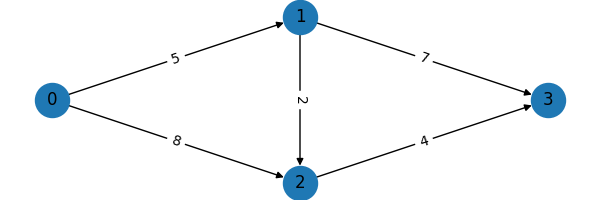
\includegraphics[scale=0.75]{primer-grafo/primer-grafo}
\end{figure}

En la \textit{sección~\ref{sec:4-tutorial_de_qiskit}} se consiguieron replicar los cálculos teóricos de una instancia de QAOA simple, sin restricciones y poco profunda.
Por ello, el siguiente problema a resolver aumenta su complejidad, añadiendo restricciones y aumentando la cantidad de qubits del sistema.

El problema, presentado en el artículo por Urgelles \textit{et al.} (2022)\cite{multi-objective_routing_optimization}, consiste en encontrar el camino más corto que conecte los nodos \textit{0} y \textit{3}.

\begin{itemize}
\item \textbf{Objetivo:}

  \begin{align}
    &\min(5X_{01} + 8X_{02} + 2X_{12} + 7X_{13} + 4X_{23}) \\
    &\textnormal{donde } X_{ij} = \begin{cases} \nonumber
      1 \textnormal{ si el camino contiene la arista del nodo \textit{i} al \textit{j}} \\
      0 \textnormal{ en otro caso}
    \end{cases}
  \end{align}
  
\item \textbf{Restricciones:}

  También se deben añadir una serie de restricciones para evitar caminos triviales o incongruentes.

  \begin{enumerate}
  \item\label{it:4-primer_grafo_restriccion_ini} $X_{01} + X_{02} = 1$:
    Debe haber exactamente un eje del camino que involucre al nodo de comienzo.
    Obliga al camino a comenzar por dicho nodo.

  \item\label{it:4-primer_grafo_restriccion_inter} $X_{01} = X_{12} + X_{13} \\
    X_{02} + X_{12} = X_{23}$:
    Para cada nodo intermedio debe haber en el resultado tantas aristas entrantes como salientes.
    Evita caminos incongruentes y hace que el único nodo posible para finalizar sea el nodo final.
  \end{enumerate}

  Siguiendo el caso del artículo\cite{multi-objective_routing_optimization} se elige el valor del modificador de Lagrange (\textit{P}) tal que sea estrictamente mayor que el máximo de la función objetivo:

  \begin{align}
    P = 1 + \max_{x}{(f_{\textnormal{sin restricc}}(X))} = 1 + \sum_{(i, j)\in{E}}{w_{ij}} = 27
  \end{align}

\end{itemize}

De acuerdo con los pasos descritos en la \textit{sección~\ref{sec:3-problemas de optimizacion combinatoria}}, la función de coste clásica en su versión QUBO es:

\begin{align}
  f(X) &= 5X_{01} + 8X_{02} + 2X_{12} + 7X_{13} + 4X_{23} + \nonumber \\
       &+ P{(X_{01} + X_{02} - 1)}^2 + P{(X_{01} - X_{12} - X_{13})}^2 + P{(X_{02} + X_{12} - X_{23})}^2
\end{align}

El número de qubits del sistema cuántico es igual a la cantidad de variables de la función de coste, esto es, la cantidad de ejes del grafo.
Por lo tanto se emplean 5 qubits.

El paso de la función a formato Ising, explicado en la \textit{sección~\ref{sec:3-operador_c}}, para la conversión de la función de coste al circuito ansatz se realiza teniendo en cuenta que las variables $X$ toman valores 0 y 1.
En este caso la correspondencia entre $X_{ij}$ y $z_k$ es la siguiente:
$X_{01}$ corresponde con $z_0$,
$X_{02}$ corresponde con $z_1$,
$X_{12}$ corresponde con $z_2$,
$X_{13}$ corresponde con $z_3$ y
$X_{23}$ corresponde con $z_4$.
\\
Estas nuevas variables $z$ van a tomar valores -1 y 1 y cada variable $z_k$ estará asociada al qubit k-ésimo del circuito. 

De acuerdo con la \textit{sección~\ref{sec:3-operador_c}} la versión Ising de la función de coste queda como:

\begin{align}
  g(z) = &5\frac{1-z_0}{2} + 8\frac{1-z_1}{2} + 2\frac{1-z_2}{2} + 7\frac{1-z_3}{2} + 4\frac{1-z_4}{2} + \nonumber \\
         &+ P{(\frac{1-z_0}{2} + \frac{1-z_1}{2} - 1)}^2 + P{(\frac{1-z_0}{2} - \frac{1-z_2}{2} - \frac{1-z_3}{2})}^2 + \nonumber \\
         &+ P{(\frac{1-z_1}{2} + \frac{1-z_2}{2} - \frac{1-z_4}{2})}^2 = \nonumber \\
  = & 11z_0 - 17.5z_1 - 28z_2 - 17z_3 + 11.5z_4 + \nonumber \\
         &+ 13.5(z_0z_1 - z_0z_2 - z_0z_3 + z_1z_2 - z_1z_4 + z_2z_3 - z_2z_4) + \nonumber \\
         &+ 80.5
\end{align}
\par
Esta igualdad solo se cumple para variables con valores \(\{-1, 1\}\), ya que \(z_i^2 = 1\).

De forma similar a la \textit{sección~\ref{sec:4-tutorial_de_qiskit}} (demostrado en la \textit{sección~\ref{CAP:F_CLASICA_A_HAMILTONIANO}} del apéndice) se obtiene el hamiltoniano $U(C, \gamma)$ a partir de $g(z)$:

\begin{align}
  &U(C, \gamma) = \exp(-i \gamma C) = \nonumber \\
  &= Rz_0(11*2\gamma) \cdot Rz_1(-17.5*2\gamma) \cdot Rz_2(-28*2\gamma) \cdot Rz_3(-17*2\gamma) \cdot Rz_4(11.5*2\gamma) \cdot \nonumber \\
  & \cdot Rz_0z_1(+13.5 * 2\gamma) \cdot Rz_0z_2(-13.5 * 2\gamma) \cdot Rz_0z_3(-13.5 * 2\gamma) \cdot Rz_1z_2(+13.5 * 2\gamma) \cdot \nonumber \\
  & \cdot Rz_1z_4(-13.5 * 2\gamma) \cdot Rz_2z_3(+13.5 * 2\gamma) \cdot Rz_2z_4(-13.5 * 2\gamma)
\end{align}

Con el operador \(U(B, \beta)\) y el vector inicial, definidos en la \textit{sección~\ref{sec:3-circuito de qaoa}}, y el operador \(U(C, \gamma)\) obtenido se puede construir el circuito cuántico.

\paragraph{Discusión de la diferencia entre circuitos de distintas implementaciones de QAOA\label{sec:4-primer_grafo_diferencias_con_el_articulo}}

\begin{figure}[Circuito {--} shortest path de Urgelles \textit{et al.} (2022) propio]{fig:4-primer_circuito}{ Circuito obtenido con la implementación de QAOA del TFG ($p=1$) }
  \centering
  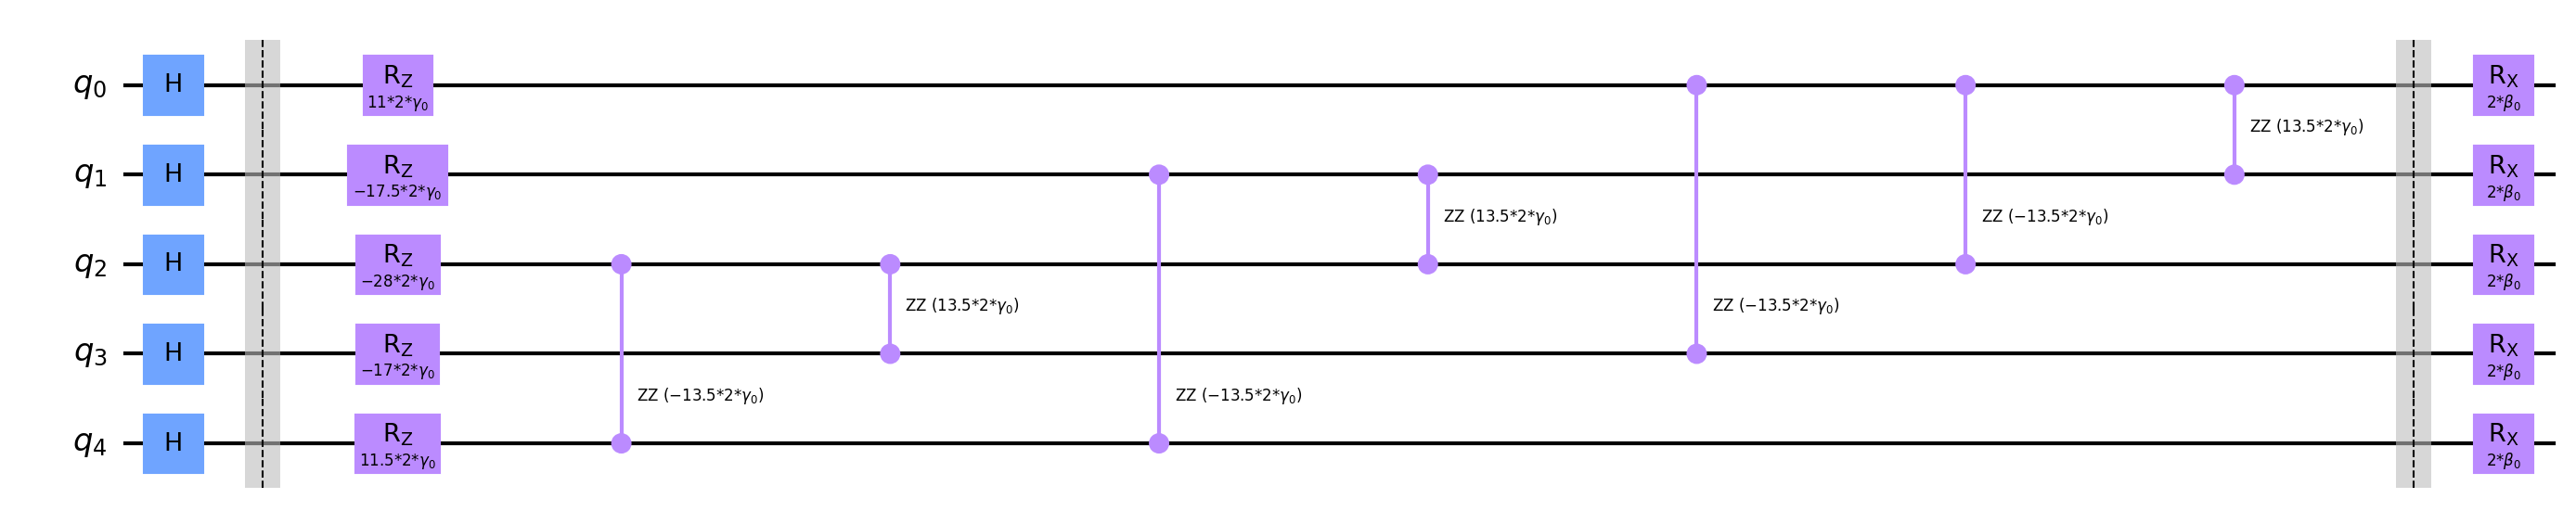
\includegraphics[scale=0.33]{circuits/primer/primer-circuit-2gamma-p1.png}
\end{figure}

\begin{figure}[Circuito {--} shortest path de Urgelles \textit{et al.} (2022) de la fuente]{fig:4-primer_paper_circuito}{ Circuito del artículo\cite{multi-objective_routing_optimization} ($p=1$) }
  \centering
  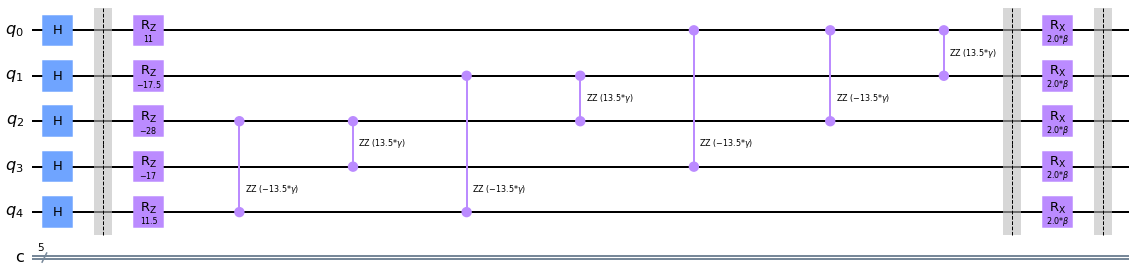
\includegraphics[scale=0.37]{circuits/paper/paper-circuit.png}
\end{figure}

\begin{figure}[Circuito {--} shortest path de Urgelles \textit{et al.} (2022) de QAOAAnsatz]{fig:4-primer_QAOAAnsatz_circuito}{ Circuito generado por QAOAAnsatz ($p=1$) }
  \centering
  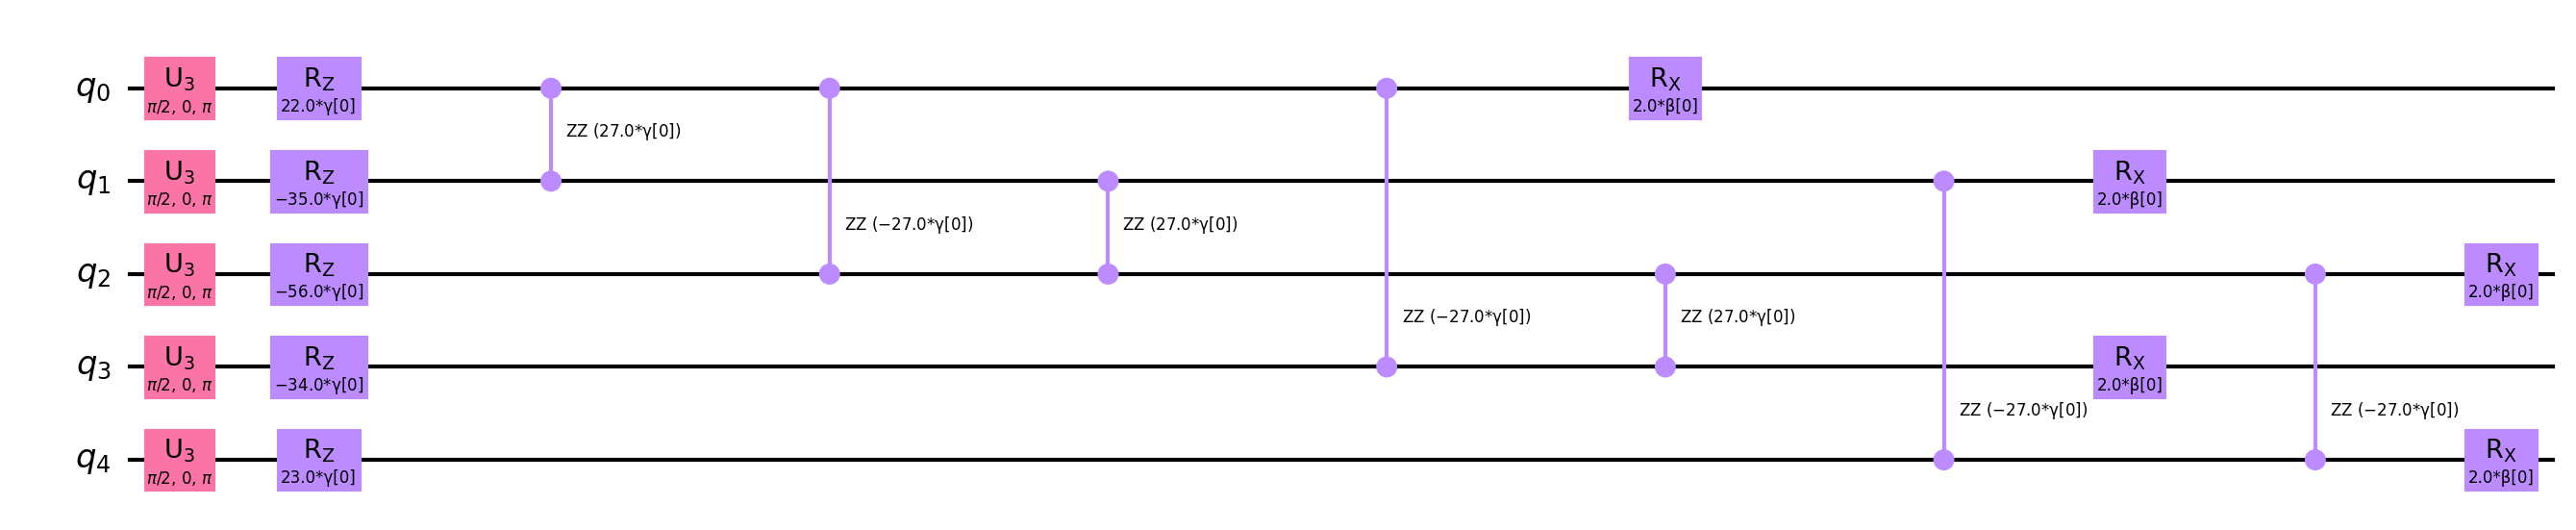
\includegraphics[scale=0.33]{circuits/primer/primer-circuit-qaoaAnsatz-p1.png}
\end{figure}

El circuito generado por la implementación propia de QAOA (\textit{fig.~\ref{fig:4-primer_circuito}}) es equivalente al generado por la función \textit{QAOA Ansatz} (fig.~\ref{fig:4-primer_QAOAAnsatz_circuito}).
El circuito generado por el artículo (fig.~\ref{fig:4-primer_paper_circuito}) sí muestra diferencias con respecto a los otros dos circuitos.

\begin{itemize}
\item Los operadores aparecen con la forma $Rzz(n), Rz(n)$ en lugar de $Rzz(n*2), Rz(n*2)$ respectivamente.
  De forma similar al problema anterior, esto no es considerado un error, ya que en el caso del artículo\cite{multi-objective_routing_optimization} se estará calculando sobre un operador $C' = \frac{C}{2}$, que tiene un mismo estado fundamental pero con la mitad de energía.

\item Las puertas $Rz$ no dependen de $\gamma$.
  Esto hace que las rotaciones llevadas a cabo por estas sean constantes lo cual, de acuerdo con el desarrollo matemático mostrado anteriormente y el resultado mostrado por la función de Qiskit que implementa QAOA, es erróneo.
  
\end{itemize}

Por esto se concluye que existe una imprecisión en la implementación del artículo y se notifica debidamente a los autores.
\\
Se han realizado pruebas utilizando ambos circuitos para realizar comparaciones y se ha comprobado que la implementación de este TFG coincide con la de la librería Qiskit.


%%% Local Variables:
%%% mode: latex
%%% TeX-master: "../tfgtfmthesisuam"
%%% End:
